
\begin{frame}{Introdução}
  
Sistema que controla o tráfego de pacotes em uma rede de acordo com
regras pré-definidas.

\begin{figure}[ht]
\centering
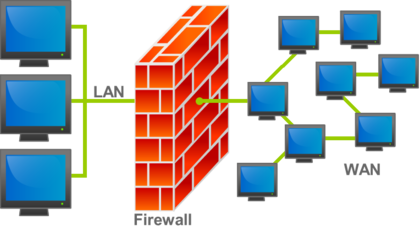
\includegraphics[scale=.7]{firewall.png}
\caption{Esquema de um firewall\footnote{\scriptsize Adaptado de
    \url{https://commons.wikimedia.org/wiki/File:Firewall.png}}.}
\end{figure}

\end{frame}

\begin{frame}{Ferramentas}

  Nos sistemas Linux o firewall normalmente utilizado é o
  \href{http://www.netfilter.org/projects/nftables/}{nftables}, e nos
  sistemas BSD, o \href{http://www.openbsd.org/faq/pf/}{pf} ({\em packet
    filter}).

\end{frame}

\begin{frame}{Regras de bloqueio}

  O firewall utiliza algumas características dos pacotes na rede,
  dentre elas:

\begin{itemize}
\item Porta de origem;
\item IP de destino;
\item Porta de destino;
\item Protocolo IP (TCP ou UDP).
\end{itemize}
\end{frame}

\begin{frame}{nftables}
\end{frame}
\begin{frame}{Cadeias}{{\it chains\/}}
\begin{tikzpicture}[node distance=2.5cm,main/.style = {draw}] 
  \node[] (ingoing) {entrada};
  \node[] (routing) [right of=ingoing] {roteamento};
  \draw[] (ingoing) -- (routing);
  \node[draw] (forward) [right of=routing] {\bf forward};
  \draw[->] (routing) -- (forward);
  \node[draw] (input) [below of=routing] {\bf input};
  \draw[->] (routing) -- (input);
  \node[draw,ellipse] (process) [below right of=input] {processos locais};
  \draw[->] (input) -- (process);
  \node[draw] (output) [above right of=process] {\bf output};
  \draw[->] (process) -- (output);  
  \node[] (outgoing) [right of=forward] {saída};
  \draw[->] (forward) -- (outgoing);
  \draw[->] (output) -- (outgoing);  
\end{tikzpicture} 
\end{frame}
